%----------------------------------------------------------------------------------------
%	PACKAGES AND THEMES
%----------------------------------------------------------------------------------------
%% Presentation presented at Blue Origin. Compiles with xelatex.


\documentclass[aspectratio=169]{beamer}

\mode<presentation> {
\usetheme{Madrid}

%\setbeamertemplate{footline} % To remove the footer line in all slides uncomment this line
%% \setbeamertemplate{footline}[page number] % To replace the footer line in all slides with a simple slide count uncomment this line

\setbeamertemplate{navigation symbols}{} % To remove the navigation symbols from the bottom of all slides uncomment this line
}

\usepackage{graphicx} % Allows including images
\usepackage{booktabs} % Allows the use of \toprule, \midrule and \bottomrule in tables
\usepackage{textcomp} % for ``reserved'' symbol

%% Bunch of stuff to make a flowchart with tikz
\usepackage{tikz}
\usetikzlibrary{shapes.geometric,backgrounds,positioning,
  positioning-plus,node-families,calc}
\tikzset{
  basic box/.style = {
    shape = rectangle,
    align = center,
    draw  = #1,
    fill  = #1!25,
    rounded corners},
  header node/.style = {
    Minimum Width = header nodes,
    font          = \strut\Large\ttfamily,
    text depth    = +0pt,
    fill          = white,
    draw},
  header/.style = {%
    inner ysep = +1.5em,
    append after command = {
      \pgfextra{\let\TikZlastnode\tikzlastnode}
      node [header node] (header-\TikZlastnode) at (\TikZlastnode.north) {#1}
      node [span = (\TikZlastnode)(header-\TikZlastnode)]
        at (fit bounding box) (h-\TikZlastnode) {}
    }
  },
  hv/.style = {to path = {-|(\tikztotarget)\tikztonodes}},
  vh/.style = {to path = {|-(\tikztotarget)\tikztonodes}},
}

%----------------------------------------------------------------------------------------
%	TITLE PAGE
%----------------------------------------------------------------------------------------

\title[Summary Presentation]{Geoff Rosenberg Interview} % The short title appears at the bottom of every slide, the full title is only on the title page

\author{Geoff Rosenberg} % Your name
\institute[] % Your institution as it will appear on the bottom of every slide, may be shorthand to save space
{
%% \medskip
\textit{Geoff.Rosenberg@gmail.com} % Your email address
}
\date{June 1, 2018} % Date, can be changed to a custom date

\begin{document}

\begin{frame}
  \titlepage % Print the title page as the first slide
\end{frame}

\begin{frame}
\frametitle{Overview} % Table of contents slide, comment this block out to remove it
\tableofcontents % Throughout your presentation, if you choose to use \section{} and \subsection{} commands, these will automatically be printed on this slide as an overview of your presentation
\end{frame}

%----------------------------------------------------------------------------------------
%	PRESENTATION SLIDES
%----------------------------------------------------------------------------------------

%------------------------------------------------
\section{Personal Summary} % Sections can be created in order to organize your presentation into discrete blocks, all sections and subsections are automatically printed in the table of contents as an overview of the talk
%------------------------------------------------

%% ** First 20 minutes of the presentation should be a high level overview of myself -- call it a personal statement.
%% **** Why am I changing jobs?
%% ***** I've always wanted to work in space
%% ***** Don't really like working for the government and having our technology being integrated by a third party

\subsection{Goals}
\begin{frame}
  \frametitle{Goal Statement}
  I want to go into the space industry because I want the world to
  benefit from the work I do.  That's why I went into renewable
  energy, and that's why I want to go into the space industry.

  \begin{figure}
    
\includegraphics[width=0.7\linewidth]{blue-origin-logo.png}
  \end{figure}
\end{frame}

\begin{frame}
  \frametitle{Interests} 
  \begin{itemize}
  \item I've always loved learning about how things work,
    and solving problems
  \item Control of autonomous systems (built robots as a kid)
  \item Control software
  \item Designing and building experiments
  \item Built model rockets as a kid and demoed them for my 5th grade
    class
  \end{itemize}
\end{frame}

\begin{frame}
  \frametitle{Motivation}
  \begin{itemize}
  \item Challenge of our time
  \item Humanity's greatest survival imperative
  \item Fermi's paradox and the Great Filter
  \end{itemize}
\end{frame}

\subsection{Undergrad}
\begin{frame}
  \frametitle{Schools}
  \begin{figure}
    
\includegraphics[width=0.35\linewidth]{USC_Logo.png}
  \end{figure}

  \begin{figure}
    
\includegraphics[width=0.35\linewidth]{ucsd-athletics-logo.png}
  \end{figure}
\end{frame}

\begin{frame}
  \frametitle{Undergrad (UCSD)}
  \begin{columns}[t]            % t for top alignment, c for centered
    \column{0.45\textwidth}
  \begin{itemize}
  \item Was and is one of the top engineering programs in the country
  \item Majored in  mechanical engineering, due to its versatility
  \item Almost went to UW
  \item Won our team robotics competition in our senior design course
  \end{itemize}

  \column{0.65\textwidth}
  \begin{figure}
    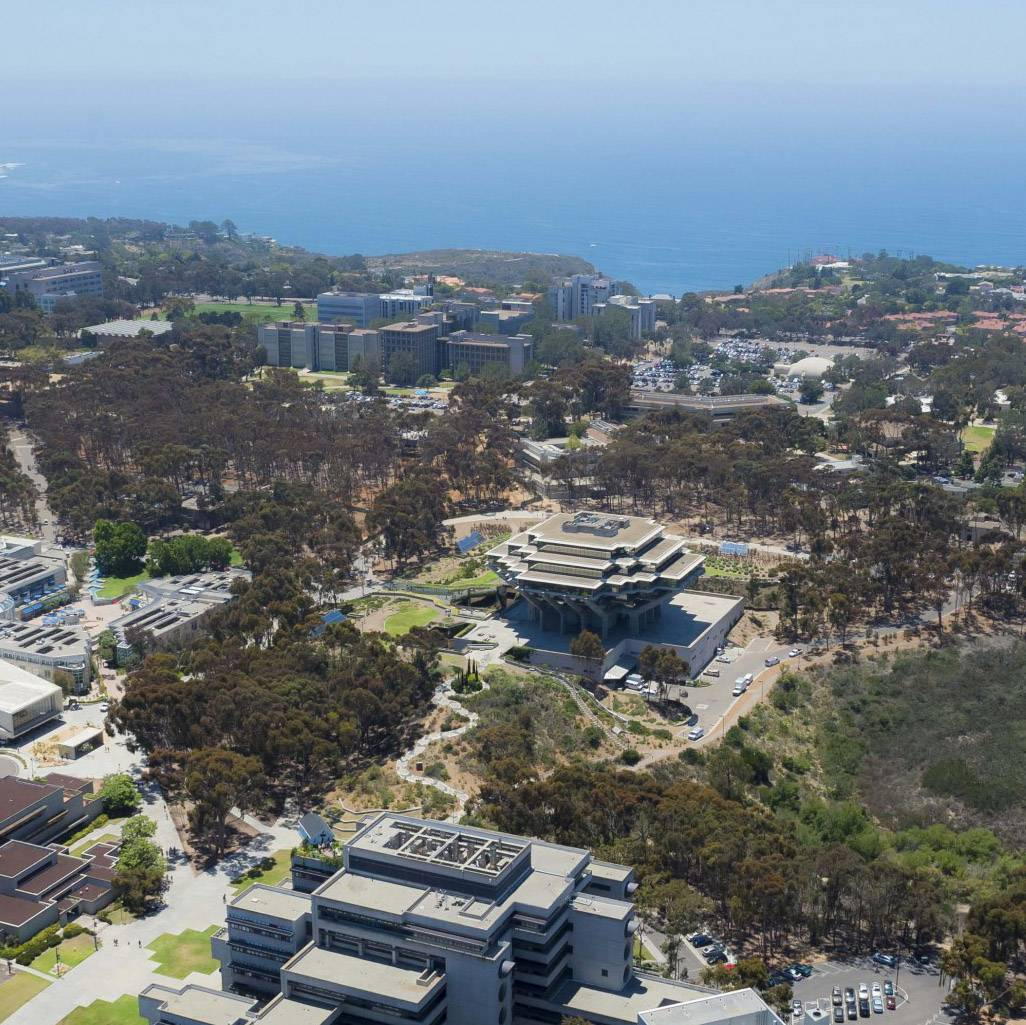
\includegraphics[width=0.7\linewidth]{UCSD.jpg}
  \end{figure}
  \end{columns}
\end{frame}

\subsection{Grad School}
\begin{frame}
  \frametitle{Grad School (USC)}
  \begin{columns}[t]
    \column{0.45\textwidth}
    \begin{itemize}
    \item Undergrad linear controls professor recommended it
    \item Very strong dynamics and controls
      program
    \item I also got to play a lot of music
    \end{itemize}

    \column{0.65\textwidth}
    \begin{figure}
      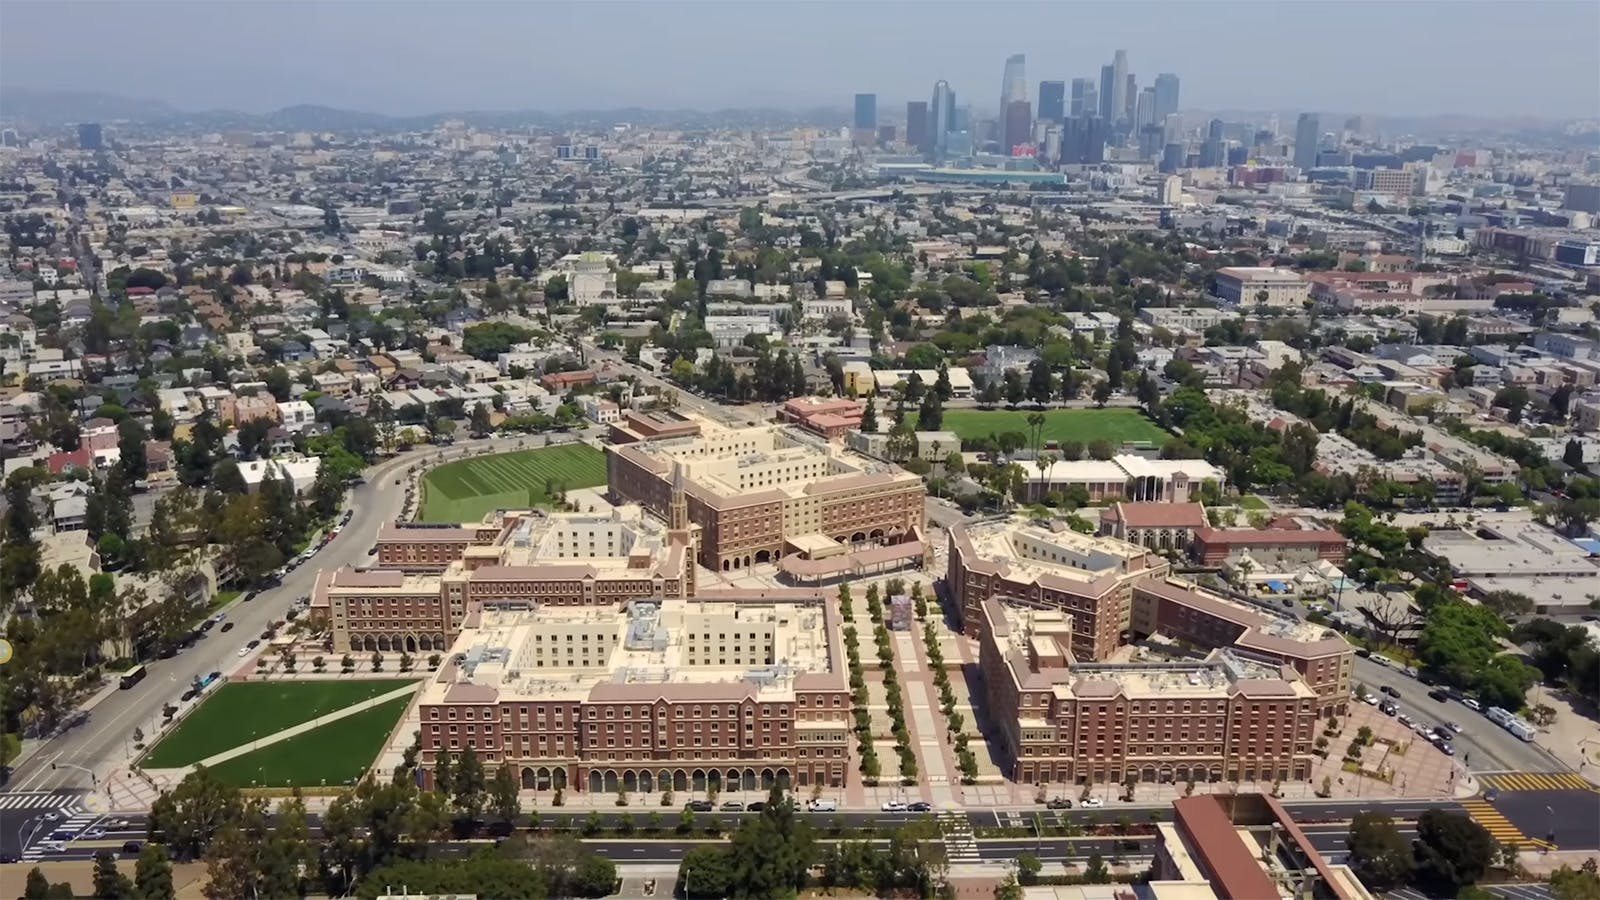
\includegraphics[width=0.7\linewidth]{USC.jpg}
    \end{figure}
  \end{columns}
\end{frame}

%------------------------------------------------
\section{Professional Career}
%------------------------------------------------

\begin{frame}
  \frametitle{Career Start -- Early 2011}
  \begin{block}{Renewable Energy}
    \begin{itemize}
      \item Challenging
      \item Interesting
      \item Beneficial to the world
    \end{itemize}
  \end{block}  
\end{frame}

\subsection{SolarReserve}
\subsubsection{Mechanical Engineer}

\begin{frame}
  \frametitle{SolarReserve}
  \center
  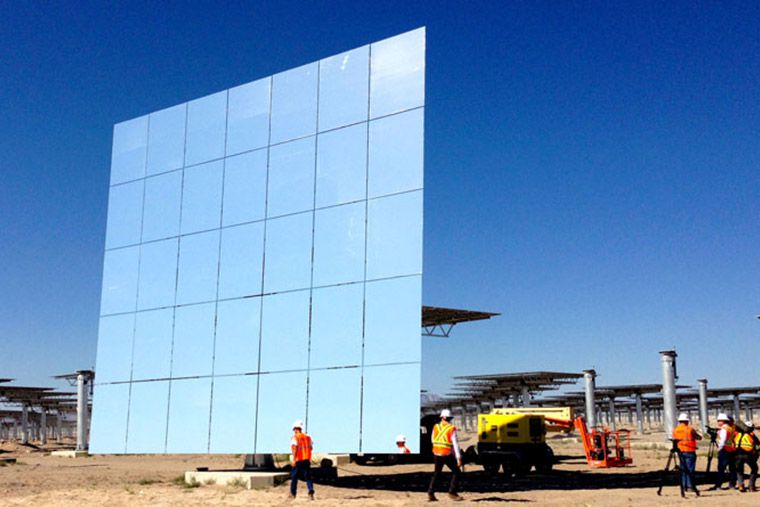
\includegraphics[width=.7\linewidth]{HeliostatImage.jpeg}
\end{frame}

\begin{frame}
  \frametitle{SolarReserve -- Summary \& Background}
  \begin{itemize}
  \item SolarReserve was founded in 2008, primarily as power project
    development company rather than a technology development company
    \begin{itemize}
    \item Exclusive worldwide license to Rocketdyne's concentrated
      solar power technology
    \item Approximately 10,000 autonomously tracking dual axis solar
      mirrors called heliostats collect energy by heating molten
      salt
    \item Thermal energy is collected during the day and stored, to
      be dispatched later as needed by the grid.
    \end{itemize}
  \item Joined SolarReserve in early 2011 as employee 64, one
    of few technical people at the company
    \begin{itemize}
    \item Came up to speed quickly as the cognizant engineer
      supporting development of photovoltaic power projects
    \end{itemize}
  \end{itemize}
\end{frame}

\begin{frame}
  \frametitle{SolarReserve -- As A Mechanical Engineer}
  \begin{itemize}
  \item Developed a photovoltaic (PV) power plant performance toolkit
    \begin{itemize}
    \item A PV performance model and design tool
    \item Enabled quick evaluation of trade studies for plant
      configuration possibilities
    \end{itemize}
  \item Worked on the plant guarantee model for our billion dollar
    Crescent Dunes power plant
    \begin{itemize}
    \item Integrated Fortran code from Rocketdyne and other
      contractors into a unified performance model
    \end{itemize}
  \item Developed and debugged the financial model used for PV
    development
    \begin{itemize}
    \item Project cash flow estimation and internal return calculation
    \end{itemize}
  \end{itemize}
\end{frame}

% PV performance model development slide
\begin{frame}
  \frametitle{SolarReserve -- Photovoltaic Design and Performance
    Evaluation Toolkit} System Design $\rightarrow$ System Performance
  $\rightarrow$ Revenue estimation $\rightarrow$ Power sale price
             [\$/MW-h]
  \begin{itemize}
  \item System design tool $\rightarrow$ Excel
  \item System performance tool $\rightarrow$ Matlab
    
    \begin{columns}[t]
      \column{0.45\textwidth}
      \begin{block}{System Design}
        \begin{itemize}
          \item Interactive tool (spreadsheet)
          \item Translates design requirements into performance tool inputs
          \item Used to generate sets of inputs for trade studies
        \end{itemize}
        
      \end{block}
      \column{0.45\textwidth}
      \begin{block}{System Performance}
        \begin{itemize}
          \item Implemented in Matlab
          \item Estimates one year of output at hourly resolution
          \item Performs data reduction and writes results into financial model
        \end{itemize}
      \end{block}
    \end{columns}
  \end{itemize}
\end{frame}

\begin{frame}
  \frametitle{Utility Photovoltaic Overview}
  \begin{columns}[t]
    \column{0.45\textwidth}
    \begin{block}{DC Components}
      \begin{itemize}
        \item Solar modules
        \item Mounting system (fixed or tracking)
        \item Low voltage circuit design
      \end{itemize}
      
    \end{block}
    \column{0.45\textwidth}
    \begin{block}{AC Components}
      \begin{itemize}
      \item Inverters
      \item Medium voltage transformers (1 - 100 kV)
      \item Generator step up transformer (100+ kV)
      \end{itemize}
    \end{block}
  \end{columns}
\end{frame}
  

\begin{frame}
  \frametitle{Photovoltaic System Design Tool}
  \begin{figure}
    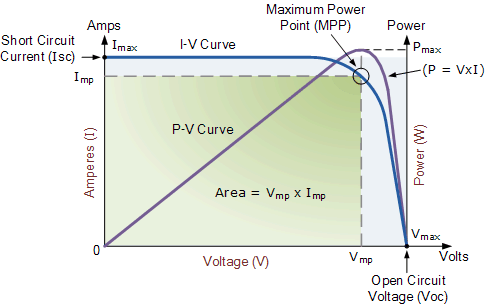
\includegraphics[width=0.25\linewidth]{IV_Curve.png}
  \end{figure}
  \begin{columns}[t]
    \column{0.45\textwidth}
    \begin{block}{Inputs (Design Characteristics)}
      \begin{itemize}
      \item Land availability
      \item Module \& Inverter electrical characteristics
      \item Interconnection voltage
      \item Row spacing
      \item Module string length
      \end{itemize}
    \end{block}

    \column{0.45\textwidth}
    \begin{block}{Outputs (Performance Tool Inputs)}
      \begin{itemize}
      \item PV performance estimation tool inputs parameters
      \item Array DC voltage and current window
      \item Estimate of land required
      \item Plant array capacity [MW$_{dc}$]
      \item Plant interconnection rating [MW$_{ac}$]
      \end{itemize}
    \end{block}
  \end{columns}
\end{frame}

\begin{frame}
  \frametitle{Design Criteria for PV Plants}
  \begin{columns}[t]
    \column{0.45\textwidth}
    \begin{block}{Financial Considerations}
      \begin{itemize}
      \item Construction time \& cost
      \item Operation and maintenance costs for different technologies
      \item Module cost and degradation rate
      \item Technology ``bankability''
      \end{itemize}
    \end{block}

    \column{0.45\textwidth}
    \begin{block}{Performance Considerations}
      \begin{itemize}
      \item AC capacity (requirement from the interconnection agreement)
      \item Module and inverter selection
      \item Fixed tilt or tracking
      \item Ratio of DC and AC capacities
      \item Ground coverage ratio
      \item Inverter MPPT Range
      \end{itemize}
    \end{block}
  \end{columns}
\end{frame}

\begin{frame}
  \frametitle{Configuring the DC System}
  \begin{block}{Electrical Requirements}
    %% \begin{columns}
    %%   \column{0.45\textwidth}
      \begin{itemize}
      \item The DC side of a photovoltaic plant block is configured
        with $n$ parallel strings of $m$ modules in series.
      \item Module $I_{max} * n <$ Inverter's DC bus current rating
        $\rightarrow$ driver for $n$
      \item Module $V_{max} * m <$ Inverter's DC bus voltage rating
        $\rightarrow$ driver for $m$
      \end{itemize}

    %%   \column{0.45\textwidth}
    %% \end{columns}
  \end{block}
  \begin{block}{Land Usage Requirements}
    \begin{itemize}
    \item Packing modules closer together vs. excessive module shading
    \item Solar trackers improve output during the morning and
      evening relative to fixed arrays, but require more space
    \end{itemize}
  \end{block}
\end{frame}

\begin{frame}
  \frametitle{Configuring the AC System}
  \begin{columns}[t]
    \column{0.65\textwidth}
    \begin{itemize}
    \item Conversion of DC power to AC through PWM.
    \item 60 Hz sinusoid (power grid frequency) broken into multiple
      steady state DC output levels
    \item Inverter carrier frequency of approximately 4 kHz
    \item Selection of the minimum DC Bus voltage tracking range
      affects the AC voltage output (Peak AC voltage = minimum DC
      tracking voltage - haircut)
    \item Design enough inverters into the plant such that there is
      enough AC capacity to cover the total output from the array
      under full sunlight
    \end{itemize}

    \column{0.45\textwidth}
    \begin{figure}
      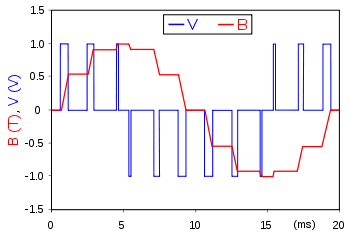
\includegraphics[width=0.75\textwidth]{PWM.png}
      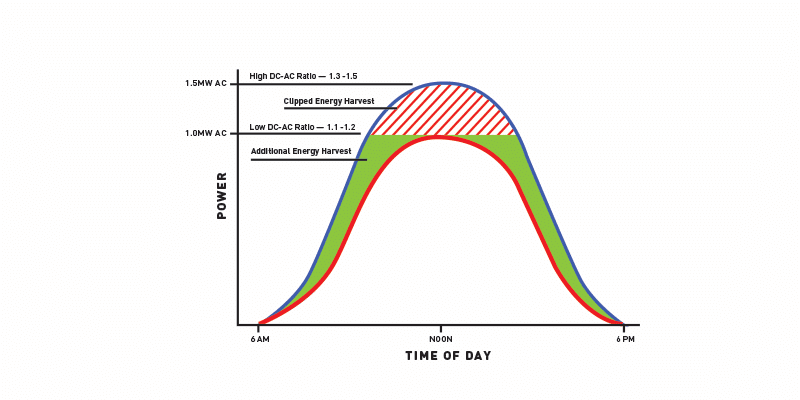
\includegraphics[width=\textwidth]{Inverter_Clipping.png}
    \end{figure}
  \end{columns}
\end{frame}

\begin{frame}
  \begin{figure}
    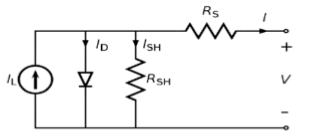
\includegraphics[width=0.3\textwidth]{Single_Diode_Model.png}
  \end{figure}
  \frametitle{PV Performance Calculation}
  \begin{itemize}
  \item Interfaces with in-house or third party implementations of a single
    diode equivalent circuit model for PV collectors
  \item Matlab code to handle calculation of gen tie losses based on
    power factor assumption, line impedance estimate, and
    interconnection voltage
  \item Optional time of day multiplier; energy delivered during peak
    demand hours is worth more to the customer
  \item Calculation of P50, P90, and P10 annual outputs, based on
    decades of hourly solar resource data
  \item Solar data available since the late 1990's,
    thanks to the NASA GOES satellites
  \end{itemize}
\end{frame}

\begin{frame}
  \frametitle{Figures of Merit for a Candidate PV Configuration}
  How we characterize the ``goodness'' of a particular configuration.
  One configuration tends not to ``fit all'' potential projects, due
  to variations in project specific constraints. 
  
  \begin{figure}
  \begin{itemize}
  \item Annual Energy Production $\rightarrow$ From performance model
  \item Performance Ratio $\rightarrow$ From performance model
  \item Specific Yield $\rightarrow$ From performance model
  \item Levelized Cost of Energy $\rightarrow$ From financial model
    \begin{itemize}
    \item All of the above items are inputs for the project financial model
    \end{itemize}
  \end{itemize}
    
    \center
    $NPV=\displaystyle\sum\limits_{t=0}^N\frac{R_{t}}{(1+d)^t}$
  \end{figure}
  
  \begin{figure}
    \raggedright
    \scriptsize
    $NPV$ - Project net present value\\
    $R_{t}$ - Net cash flow at time $t$ ($Energy*Sale Price$)\\
    $d$ - Discount rate\\
    $t$ - Time of the cash flow
  \end{figure}
\end{frame}

%% CSP Technology overview
\begin{frame}
  \frametitle{CSP Technology}
  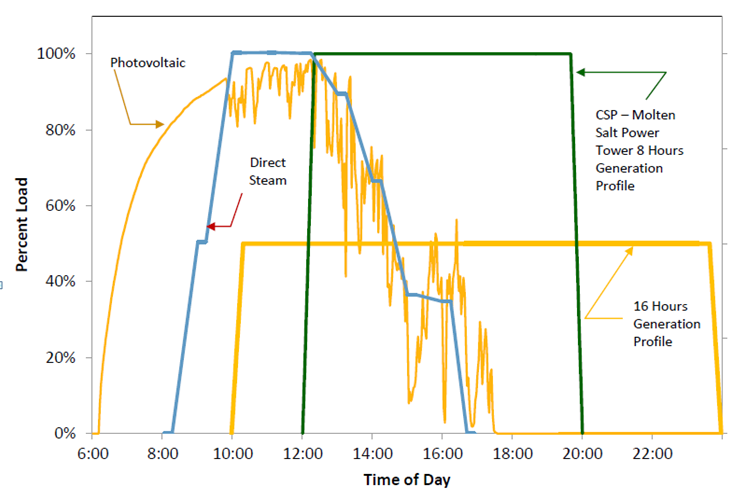
\includegraphics[width=0.75\linewidth]{PV_CSP_Profiles.png}
\end{frame}

\begin{frame}
  \frametitle{CSP Performance: Flux Model}
  Development of a Monte Carlo ray tracer to estimate the performance
  of a CSP plant's collector field based on the level of solar
  irradiation

  \begin{columns}[t]
    \column{0.45\textwidth}
    \begin{itemize}
    \item Forms the basis for the CSP performance model
    \item $E_{Grid}= SolarIntensity * A_{Glass} * \eta_{CollectorField} * \eta_{Receiver} * \eta_{Rankine}$
    \item Ray tracing engine written in Fortran
    \item Visualization tools written in Matlab
    \item Determines the heliostat kinematics for each heliostat in
      the field, and performs ray tracing
    \end{itemize}

  \column{0.45\textwidth}
  \begin{figure}
    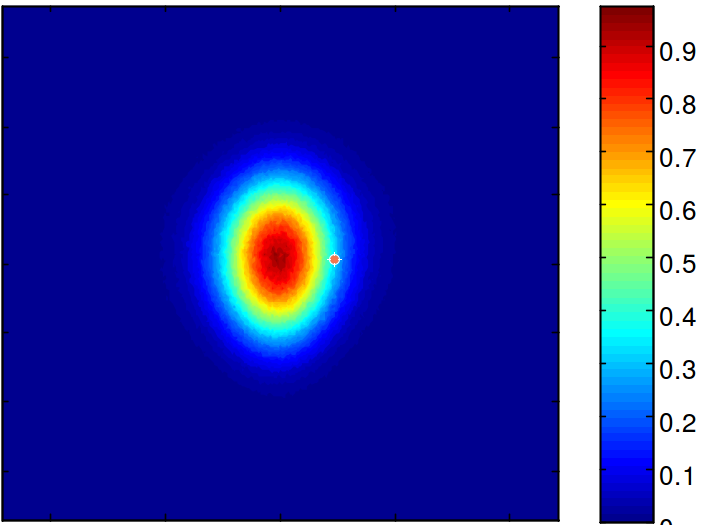
\includegraphics[width=\textwidth]{Flux_Image.png}
  \end{figure}
  \end{columns}
\end{frame}

\subsubsection{Systems Engineer}
\begin{frame}
  \frametitle{As A Systems Engineer}
  Transferred from the project to product development group in early 2014.
  \begin{itemize}
  \item Development of the real time distributed control software
  \item Development of interface software
  \item Determination and definition of performance requirements
  \item Test campaigns design
  \item Test data reduction
  \end{itemize}
\end{frame}

\begin{frame}
  Revolutionary heliostat design
  \frametitle{SR-120 Heliostat Development}
  \begin{itemize}
  \item Development of a new and disruptive type of heliostat design
  \item Fully wireless power and communication
    \begin{itemize}
    \item NiFe batteries and ZigBee communication
    \end{itemize}
  \item Two orders of magnitude smaller than conventional heliostats
    \begin{itemize}
    \item On the order of one million per plant $\rightarrow$ mass
      production becomes a possibility
    \end{itemize}
  \item Optically controlled, with central camera controller in the
    tower
  \end{itemize}
  %% My involvement on this project was chiefly the development of all
  %% software interfaces between the Matlab software and the hardware it
  %% controlled.  I was also involved in I\&T and debugging the Matlab
  %% code.
\end{frame}

%% Slide on the SR-120 software development
\begin{frame}
  \frametitle{SR-120 Heliostat Development -- Control Software}
  Distributed control logic with optical feedback
  \begin{itemize}
  \item Architecture involved both open loop and closed loop
    components to reduce communication bandwidth requirement
  \item Adaptation of an MIT thesis for open loop component
  \item Computer vision code developed to reliably identify optical
    elements on the body of the heliostats
    \begin{itemize}
    \item Maximum likelihood estimation achieved through an extended
      Kalman filter
    \end{itemize}
  \item Chiefly written in Matlab, with hardware drivers written in
    C++/CLI and C\#
  \item AGILE development philosophy
  \end{itemize}
\end{frame}

\begin{frame}
  \frametitle{SR-120 Heliostat Development -- Control Software \& Interfaces}
  Camera Interfaces and AMS software
  \begin{itemize}
  \item SR-120 control software developed in object oriented Matlab
  \item Hardware vendors frequently provide a C API as an interface
  \item Developed .NET assemblies to act as ``middleware'' between
    the SR-120 control software and the hardware
    \begin{itemize}
    \item Camera
    \item Heliostat control assembly hardware
    \end{itemize}
  \end{itemize}
\end{frame}

\begin{frame}
  \frametitle{In-Situ Heliostat Characterization at Crescent Dunes}
  \begin{columns}[t]
    \column{0.5\textwidth}
    \begin{itemize}
    \item Development of a method to characterize heliostat
      performance en masse in the field.
    \item Heliostat optical performance is the main contributor to
      field efficiency ($\eta_{CollectorField}$)
    \item Measurement of the ``bending'' heliostats to determine the
      deformation of the mirror figure and its ultimate effect on
      plant revenue
    \item Heliostat performance measurement using previously existing
      methods was slow, error prone, and labor intensive
    \end{itemize}
    \column{0.5\textwidth}
    \begin{figure}
      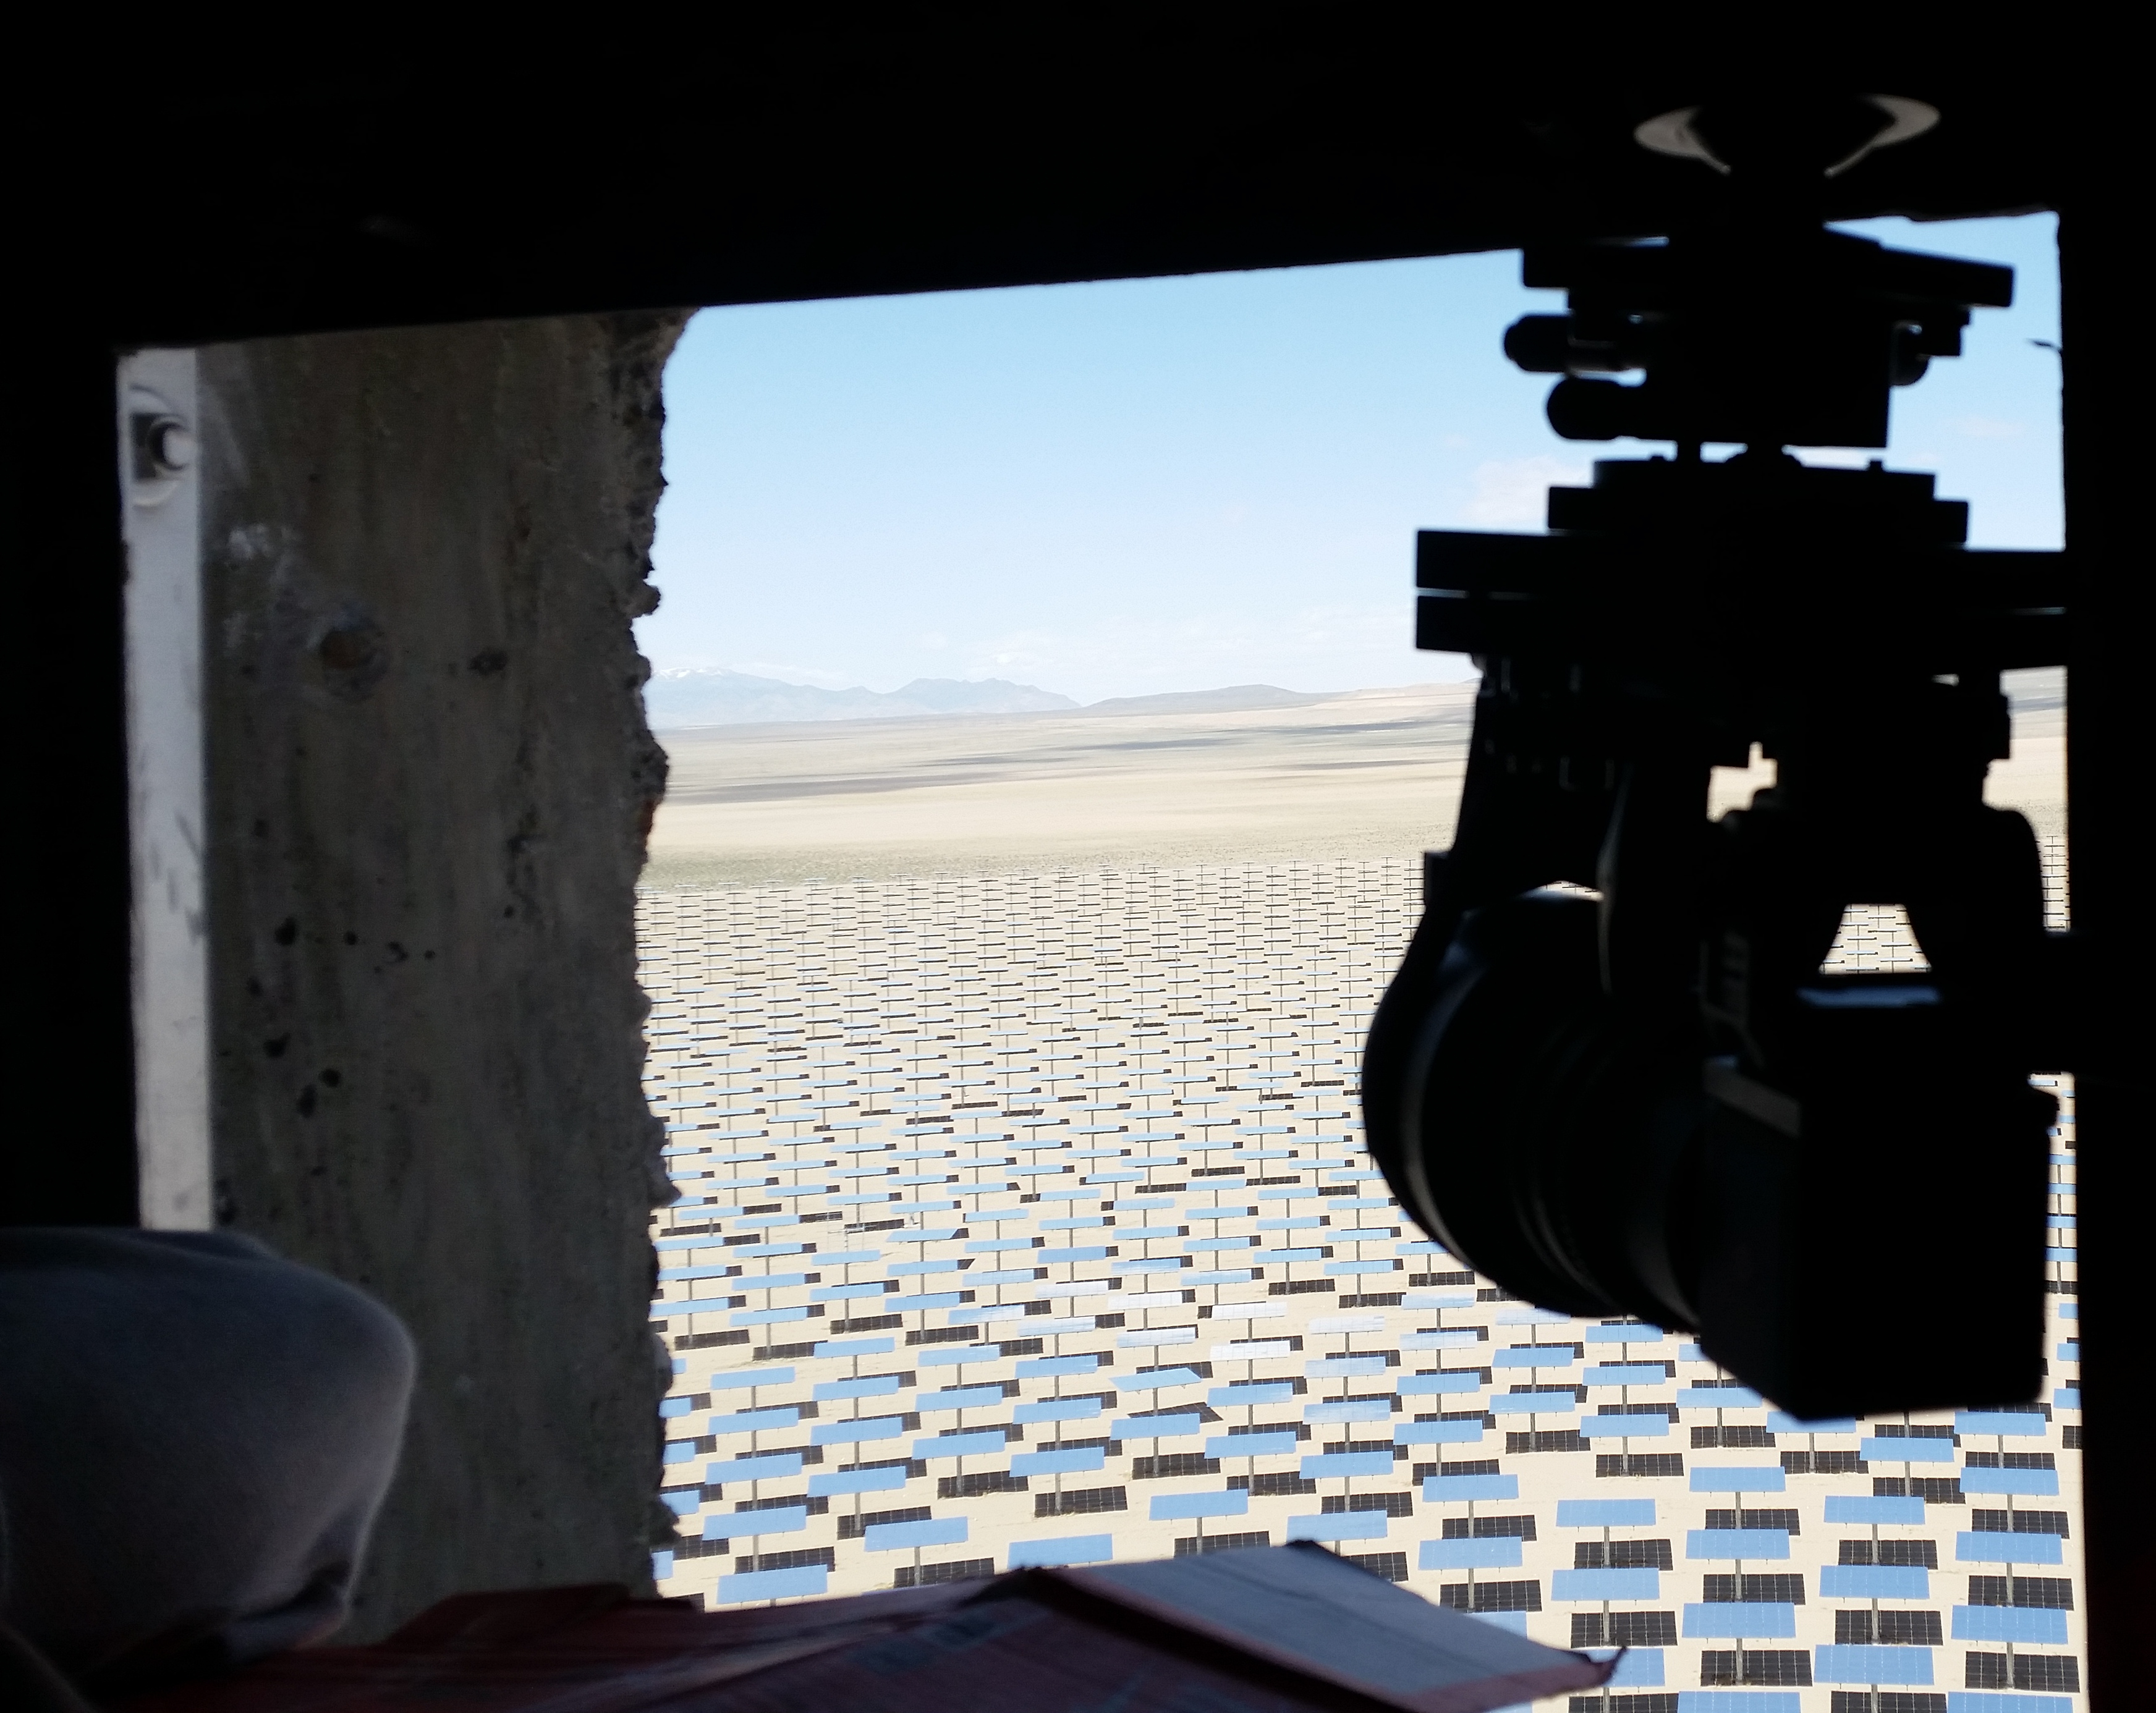
\includegraphics[width=\textwidth]{In_Situ_View.jpg}
    \end{figure}
  \end{columns}
\end{frame}

\begin{frame}
  \frametitle{In-Situ Heliostat Characterization -- Experiment Design}
  Design a test campaign to characterize the performance of the
  full field of 10,347 heliostats at CDSEP
  \begin{itemize}
  \item Images of the heliostats are captured at night, when the
    collector field is not operating
  \item The heliostats are articulated through their normal range of
    motion
  \item The reflection of starlight in the heliostats is captured
  \item Surface errors in the heliostats are inferred from the delta
    in pixel location between where the star's reflection is expected
    to be, and where it actually is
  \end{itemize}
\end{frame}

%% HabConnect relational database interface to write to the SCADA system's database
\begin{frame}
  \frametitle{In-Situ Characterization -- Software Development}
  \begin{itemize}
  \item Re-used large amounts of code originally developed for the SR-120
  \item CDSEP main field control system runs in GE Grid eTerra environment
    \begin{itemize}
    \item Necessitated an interface between the main plant control
      system's database and our Matlab software
    \item Utilized the C API provided by GE Grid
    \end{itemize}
  \end{itemize}
\end{frame}

%% HabConnect relational database interface to write to the SCADA system's database
\begin{frame}
  \frametitle{In-Situ Characterization -- Hardware Development}
  \begin{figure}
    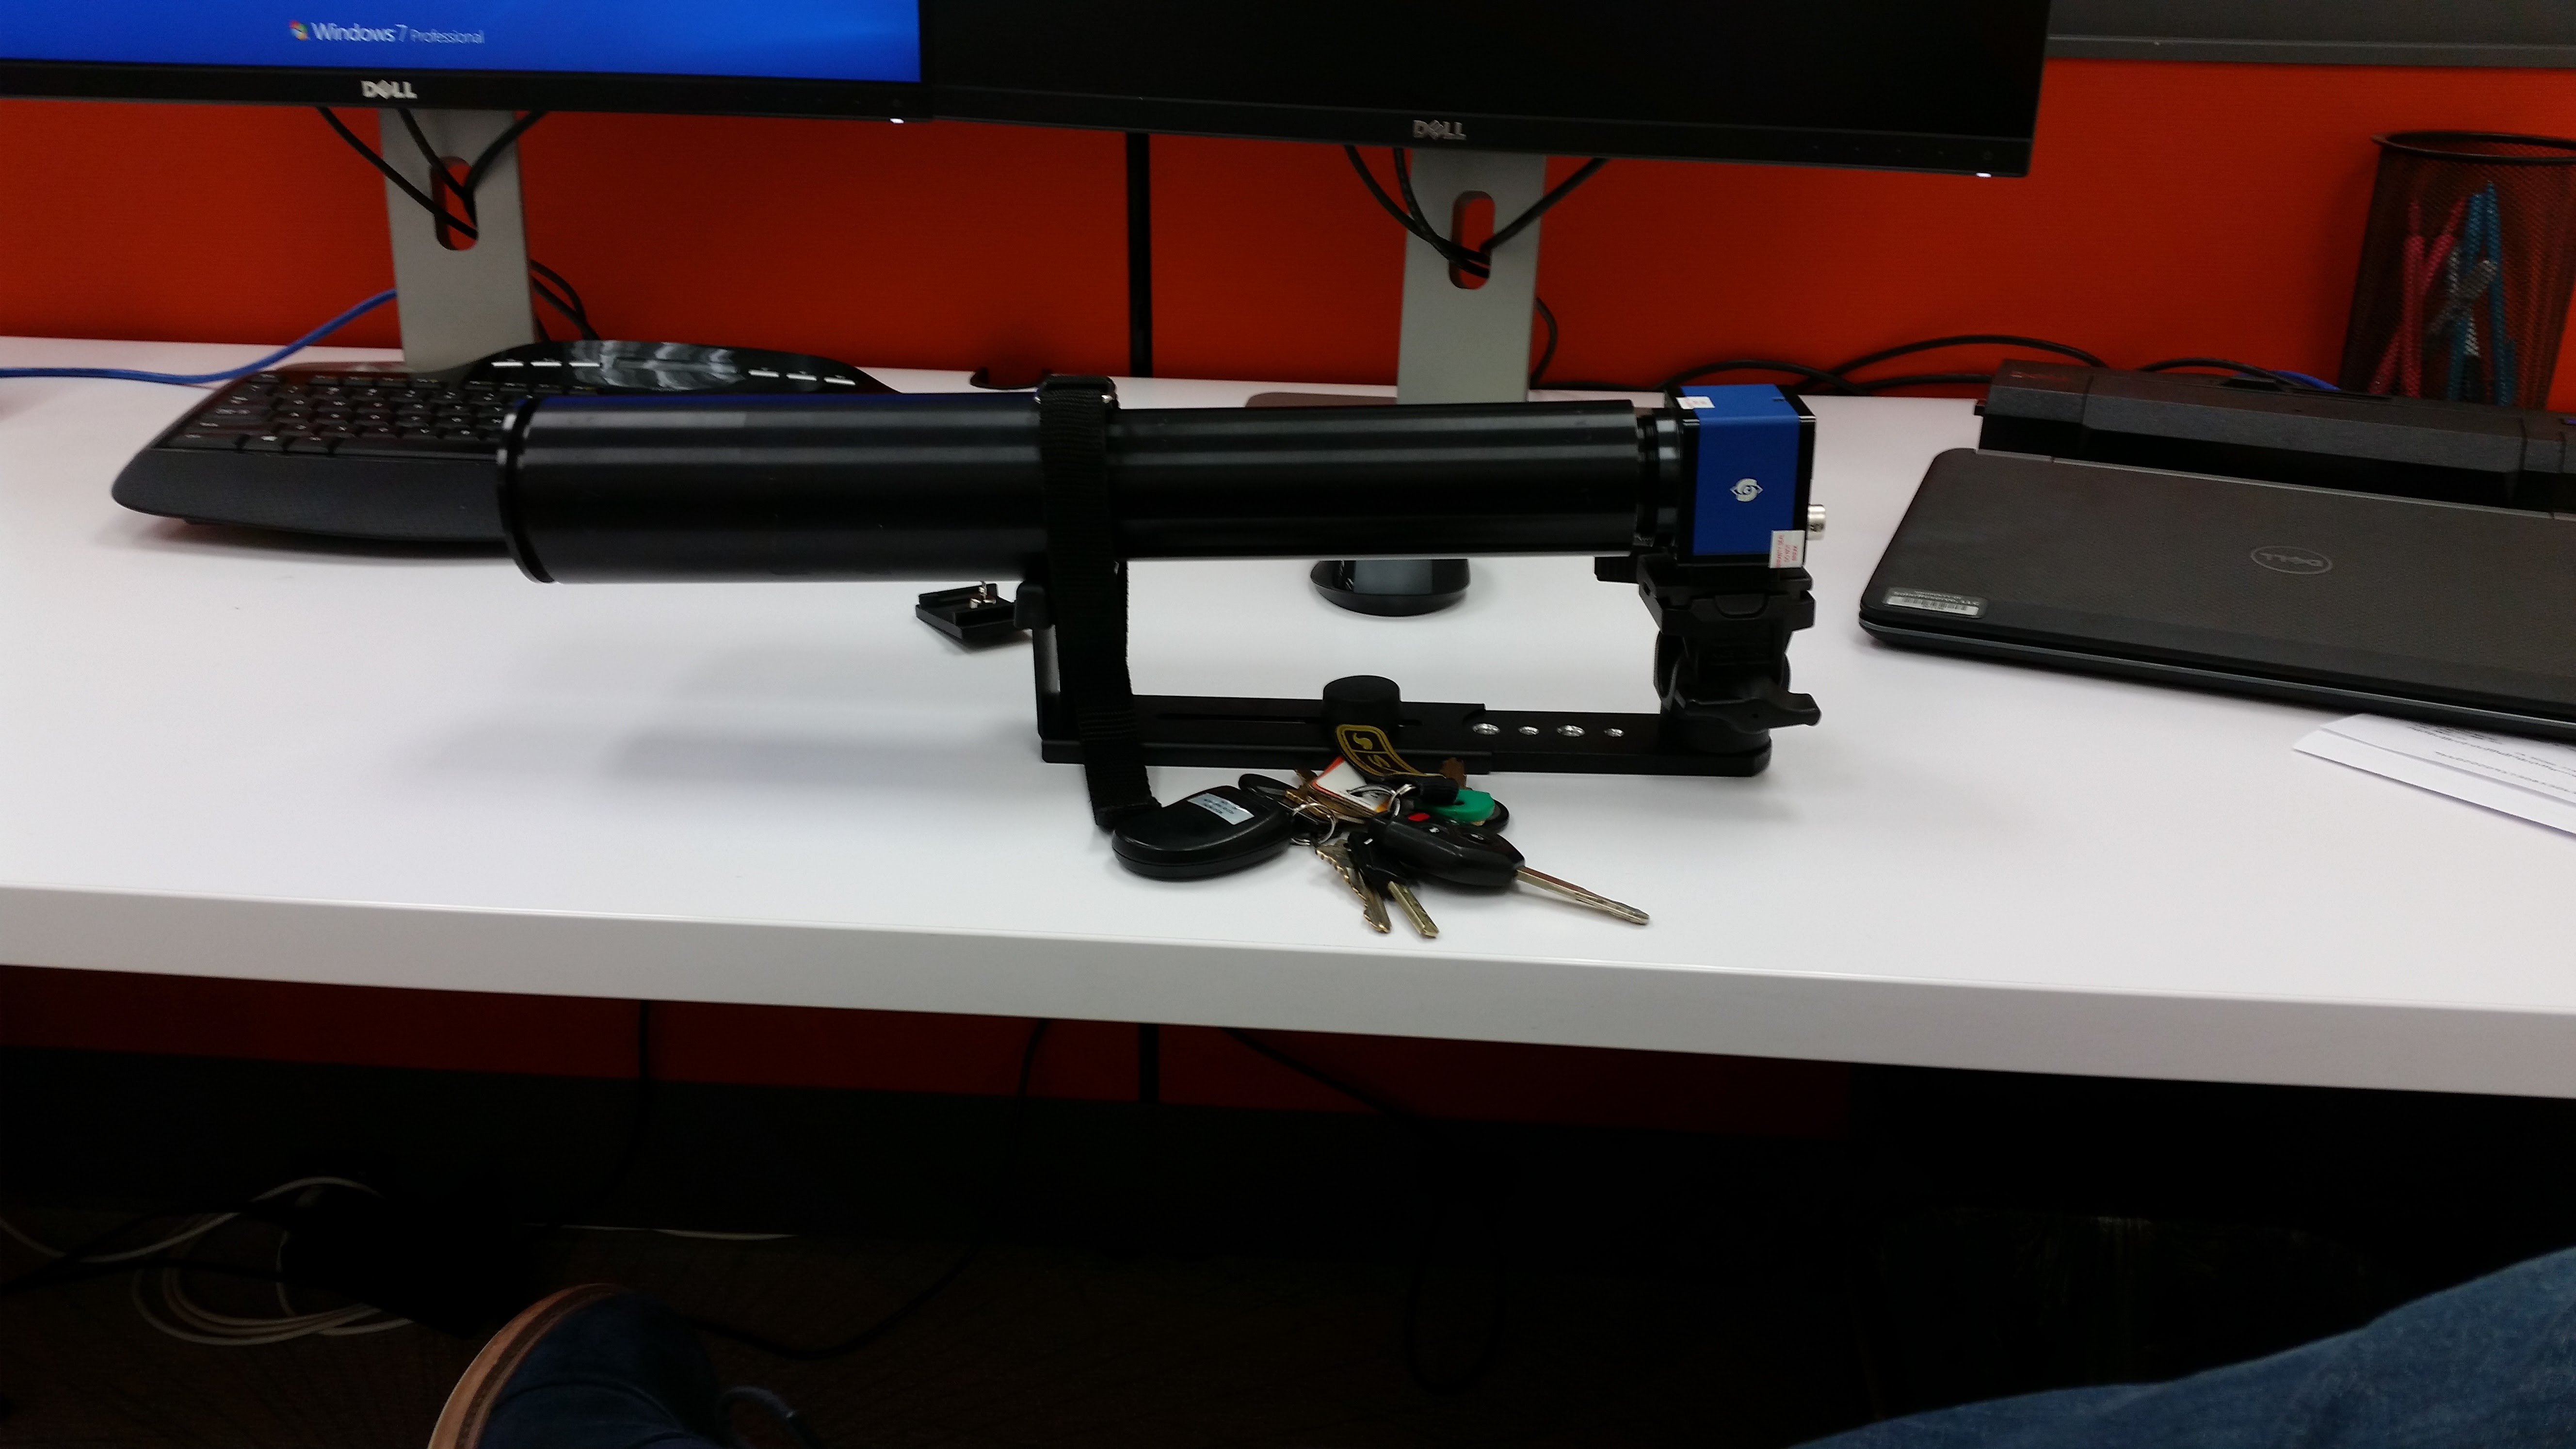
\includegraphics[width=0.5\textwidth]{CameraMount.jpg}
  \end{figure}
  \begin{itemize}
  \item Nighttime testing campaigns involved mounting a camera to the
    CDSEP tower at night
  \item Detachable, allowing it to be stowed during daytime operation of the plant
  \item Repeatable to sub milliradian accuracy
  \item Assembled from Thorlabs components for precision motion control
  \item Went through several desktop iterations before field testing it
  \end{itemize}
\end{frame}

%% All of the testing campaigns at SNL
\begin{frame}
  \frametitle{Integration and Test -- Sandia}
  \begin{columns}[c]
    \column{0.5\textwidth}
    \begin{figure}
      \textbf{Solar Thermal Test Facility\\Sandia National Labs
        (Albuquerque, NM)}
      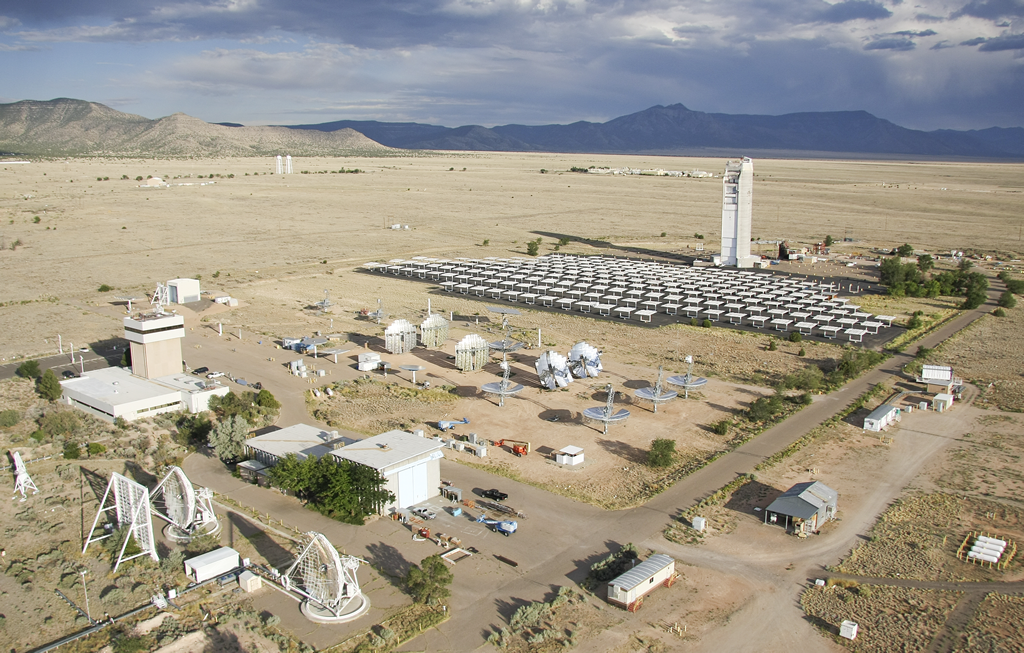
\includegraphics[width=\linewidth]{Sandia.png}
    \end{figure}

    \column{0.5\textwidth}
    \begin{itemize}
    \item Field testing of SR-120 hardware and software occurred at
      Sandia National Labs
    \item Initial field testing of the In-Situ characterization system
      did as well
    \item Much of this testing occurred remotely, controlling the
      hardware in Albuquerque from Santa Monica
    \item Experiment design, and several trips over the years for
      field testing
    \end{itemize}
  \end{columns}
\end{frame}

\begin{frame}
  \frametitle{Integration and Test -- Crescent Dunes}
  \begin{columns}[c]
    \column{0.5\textwidth}
    \begin{figure}
      \textbf{Crescent Dunes Solar Thermal Power Plant\\
        (Tonopah, NV)}
      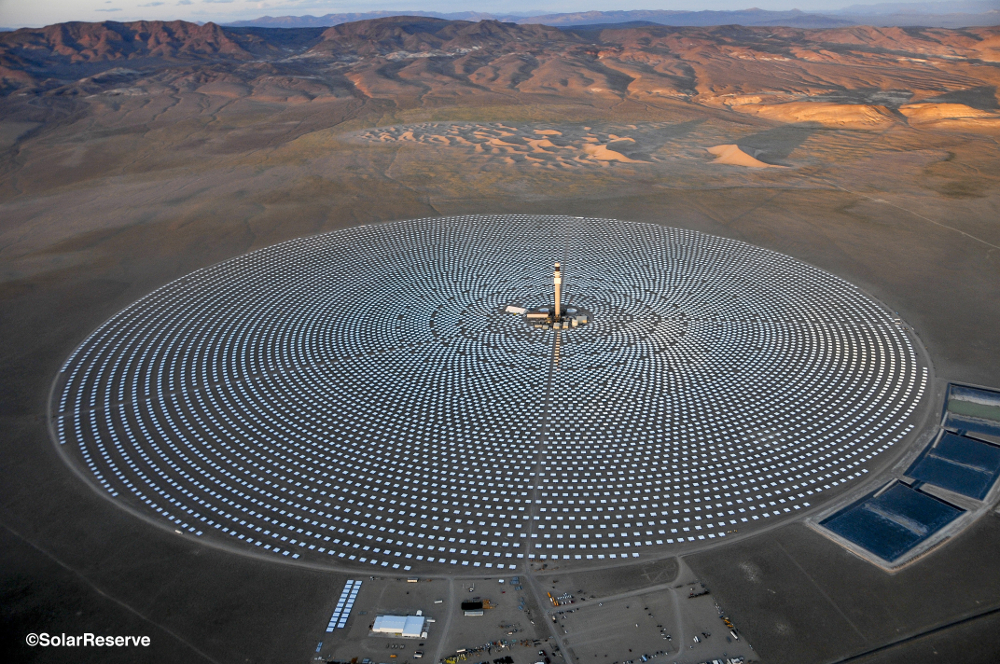
\includegraphics[width=\linewidth]{CDSEP.jpg}
    \end{figure}

    \column{0.5\textwidth}
    \begin{itemize}
    \item Most testing of the In Situ characterization software
      occurred at Crescent Dunes
    \item Challenges setting up the testing in an operating power
      plant/construction zone
    \end{itemize}
  \end{columns}
\end{frame}

\begin{frame}
  \frametitle{Integration and Test -- Raymer Test Facility}
  \begin{columns}[c]
    \column{0.5\textwidth}
    \begin{figure}
      \textbf{Raymer Test Facility\\
        (Van Nuys, CA)}
      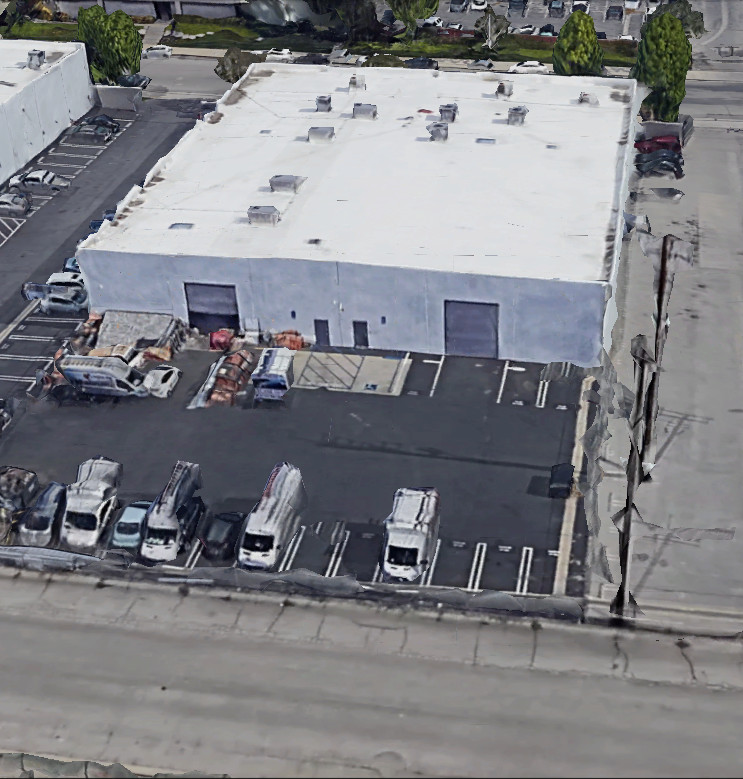
\includegraphics[width=\linewidth]{Raymer.jpg}
    \end{figure}

    \column{0.5\textwidth}
    \begin{itemize}
    \item Preliminary testing for In Situ characterization
    \item Short-range testing for the SR-120
    \end{itemize}
  \end{columns}
\end{frame}

\subsection{Lockheed}
\begin{frame}
  \frametitle{Lockheed Martin Missiles and Fire Control}
  \center
  
\includegraphics[width=.7\linewidth]{LockheedLogo}
\end{frame}

%reasons for transition
\begin{frame}
  \frametitle{Transitioning from SolarReserve}
  \begin{itemize}
  \item Lack of new contracted power projects
  \item Concerns about R\&D budget cuts
  \item Interest in applying control theory in an aerospace setting
  \end{itemize}
\end{frame}

\subsubsection{Applied Research}

\begin{frame}
  \frametitle{Affordability Test Bed}
  \begin{itemize}
  \item Small lab at the MFC Innovation center
  \item Evaluation of COTS components and substituting them into
    existing designs
  \item Most simulations run involve development in Simulink, and
    deployment to embedded hardware via Matlab auto-code
  \item Components in the lab
    \begin{itemize}
    \item Optical Bench
    \item 3D Printer
    \item Image generator
      \begin{itemize}
        \item Big computer with lots of graphics cards --
          renders images very quickly to a screen on the bench
        \item Uses a UDP client/server architecture to ensure that it
          stays ``in step'' with the running simulation
      \end{itemize}
    \item Flight computer running on a TI AM5728 chip set (Arm Cortex--A15)
    \end{itemize}
  \end{itemize}
\end{frame}


\begin{frame}
  \frametitle{Loitering Munition Simulation Overview}
  %% Describe the loitering munition simulation
  %% All lower level stuff (frame handling, hardware interfaces) is written by hand in c++.  This is what I worked on.
  \begin{itemize}
  \item Continuous time simulation of a loitering munition
    \begin{itemize}
    \item Computer vision -- on board camera sends live images back to the user
    \item Simulation of a fixed wing drone with either explosives or EMP on it
    \item Semi-autonomous
      \begin{itemize}
      \item User gets the target in the camera's FOV, designates
        it with a tablet, and lets the autopilot take over.
      \end{itemize}
    \end{itemize}
  \end{itemize}
    \begin{figure}
      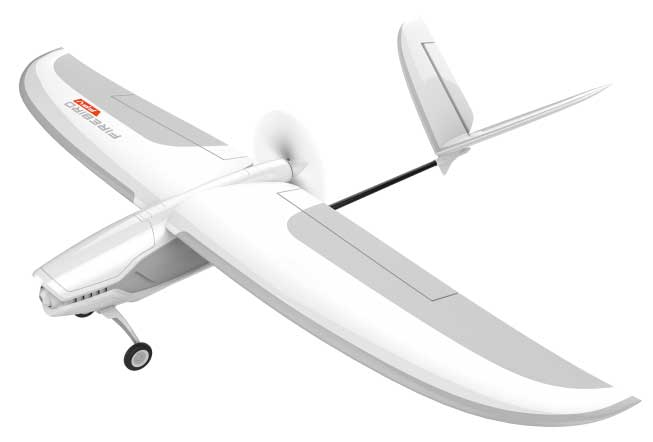
\includegraphics[width=0.4\textwidth]{Firebird-FPV-Fixed-Wing-Drone.jpg}
    \end{figure}
\end{frame}

\begin{frame}
  \frametitle {Loitering Munition Overview -- Continued}
  \begin{itemize}
  \item High level simulation and flight computer software 
  \item Written in Simulink and autocoded to C++ for deployment on the AM5728
  \item Simulation running on a Linux PC (Redhat) host
  \item My first task -- adapted the simulation to work with a different airframe
  \item My second task -- solution of the frame delay problem
  \end{itemize}
\end{frame}

\begin{frame}
  \frametitle{Loitering Munition -- Frame Delay Problem}
  \begin{itemize}
  \item Non-zero latency between the $n^{th}$ update of the simulation
    state (simulation time $t_{n}$) and when the image is rendered on
    the screen ($t_{n+\delta}$)
    \begin{itemize}
    \item Communication latency between the simulation host and image
      generator
    \item Image rendering time
    \end{itemize}
  \item Images are received by the flight computer in order, but delayed
  \item Image tracker receives frame n, but has simulation state information for frame n+1
  \item Causes erratic performance of the camera motion compensation
    code
    \begin{itemize}
    \item This problem worsens with shorter time constant (IE faster)
      munitions
    \end{itemize}
  \end{itemize}
\end{frame}

\begin{frame}
  \frametitle{Loitering Munitions -- Frame Delay Solution}  
  \begin{columns}[t]            % t for top alignment, c for centered
    \column{0.45\textwidth}
    \begin{figure}
      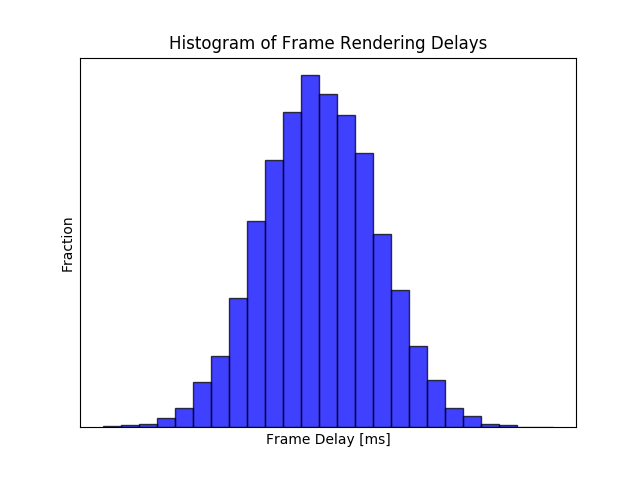
\includegraphics[width=\textwidth]{DelayHistogram.png}
    \end{figure}
    
    \column{0.45\textwidth}
    \begin{itemize}
    \item Software frame number overlay generation using the image
      generator's API with CIGI messaging
    \item Open source optical character recognition library utilized
      to read frame numbers off the screen
      \item $\delta=t_{Image Capture} - t_{Simulation}$
    \end{itemize}
  \end{columns}
\end{frame}

\begin{frame}
  \frametitle{Loitering Munitions -- Frame Delay Solution (Continued)}
  \begin{columns}[t]
    \column{0.45\textwidth}
    \begin{figure}
      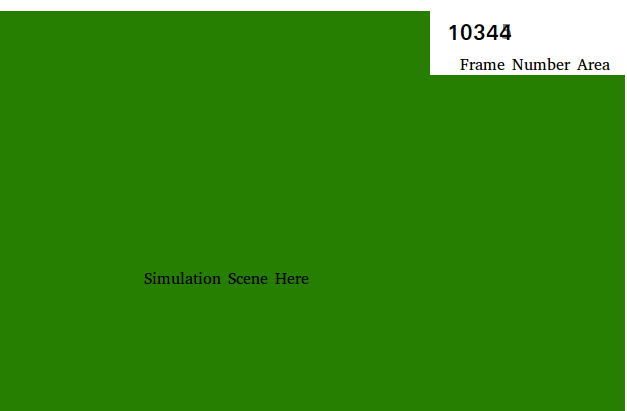
\includegraphics[width=\textwidth]{DemoLMSFrame_Corrupt.png}
    \end{figure}
    
    \column{0.45\textwidth}
  \begin{itemize}
      \item Camera triggering using vertical sync pulses
      \begin{itemize}
      \item IG display port $\rightarrow$ DVI $\rightarrow$ HDMI
        $\rightarrow$ VGA $\rightarrow$ BNC 5 wire (RGB + HSYNC + VSYNC)
        $\rightarrow$ Alligator clips $\rightarrow$ Camera
      \end{itemize}
    \item Oscilloscope testing to determine sync pulse voltage and frequency
    \item Tested the camera's hardware triggering with a waveform generator
      before installing the hardware on the bench    
  \end{itemize}
  \end{columns}
\end{frame}

%% Image injection/projection flow charts
%define some colors for the blocks
\definecolor{light_blue}{RGB}{2,127,237}

%% color definitions for the different signals
\definecolor{Ethernet}{RGB}{5,163,0}        %green
\definecolor{HDMI}{RGB}{163,111,0}   %gold
\definecolor{USB}{RGB}{0,0,255}
\definecolor{Data}{RGB}{0,0,0}

\begin{frame}
  \frametitle{Loitering Munition -- Image Projection Data Flow}
\begin{tikzpicture}[node distance = 0.6cm, thick, nodes = {align = center},
    >=latex]
  %% simulation host
  \node[fill = light_blue] (6_DOF)
       {6DOF state @\\$t_{n}$};
  \node[fill = light_blue, below = of 6_DOF] (Cigi_Cmds)
       {Cigi Update Commands};
  \node[fill = light_blue, below = of Cigi_Cmds] (Frame_Logger)
       {Frame Logger};
  \node[fill = light_blue, below = of Frame_Logger] (PNG)
       {Images Saved as PNG};
  \node[fill = light_blue, right = of PNG] (Timestamp_Log)
       {Logging of time stamps\\and file names};
  \node[fill = light_blue, left = 1.5 of PNG] (Update_Log)
       {Cigi Update Log\\$t_n$, Frame Number};
  \node[fill = light_blue, above = 1.25 of 6_DOF] (Monitor)
       {Monitor};

  %% Image generator
  \node[fill = light_blue, left = 4 of 6_DOF] (Scene_Render)
       {Scene\\Rendering};

  %% Flight computer
  \node[fill = light_blue, right = 1.5 of Cigi_Cmds] (Image)
       {Image Received @\\$t_{n+\delta}$};
  \node[fill = light_blue, above = 1.25 of Image] (Camera)
       {Camera};

  %background nodes to separate out the computers
  \begin{scope}[on background layer]
    \node[fit = (6_DOF)(Cigi_Cmds)(Frame_Logger), basic box = red,
      header = Simulation Host] (Host) {};

    \node[fit = (Scene_Render), basic box = blue,
      header = Image Generator] (Image_Generator) {};

    \node[fit = (Image)(Camera), basic box = blue,
      header = Flight Computer] (Flight_Computer) {};
  \end{scope}

  %% paths to connect the nodes
  \path[very thick, Data] (6_DOF.south) edge[->] (Cigi_Cmds.north);
  \path[very thick, Ethernet] (Cigi_Cmds) edge[->] (Scene_Render);
  \path[very thick, Data] (Cigi_Cmds) edge[->] (Update_Log);
  \path[very thick, HDMI] (Scene_Render) edge[->] (Monitor.west);
  \path[very thick, HDMI] (Monitor.east) edge[->] (Camera.west);
  \path[very thick, USB] (Camera.south) edge[->] (Image);
  \path[very thick, Ethernet] (Image) edge[->] node[pos=0.35, sloped, above] {Image Data} (Frame_Logger);
  \path[very thick, Data] (Frame_Logger) edge[->] (Timestamp_Log);
  \path[very thick, Data] (Frame_Logger) edge[->] (PNG);
\end{tikzpicture}
\end{frame}

\subsubsection{Air \& Missile Defense}

\begin{frame}
  \frametitle{Transfer to AMD}
  \begin{block}{Air \& Missile Defense}
    \begin{itemize}
      \item Lockheed line of business involved in selling missile
        defense systems
      \item Responsible for most revenue generation for Missiles \&
        Fire Control
    \end{itemize}
  \end{block}
\end{frame}

\begin{frame}
  \frametitle{PAC-3} % I might want to be a little sparing in my descriptions here, because this stuff is classified
  \begin{columns}[t]
    \column{0.5\textwidth}
  \begin{itemize}
  \item Work on a Linux computing cluster on a continuous time
    simulation
  \item Integrating changes to the simulation from internal
    contributors, and also from the simulation integrator (US Army),
    as well as the manufacturer of the ground system components
  \item Modularization of an older version of the simulation (entirely
    Fortran/Linux based) into several libraries which the customer can
    link together
  \item Runs on Windows or Linux
  \end{itemize}

  \column{0.5\textwidth}
  \begin{figure}
    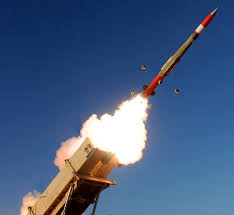
\includegraphics[width=\textwidth]{PAC-3.jpeg}
  \end{figure}
  \end{columns}
\end{frame}

\begin{frame}
  \frametitle{Configuration Management on PACNET}
  \begin{itemize}
  \item Handling configuration management on a simulation of about
    800,000 SLOC
  \item Handling requests for modification
  \item Installing new releases of our code
  \item Handling updates from the US Army
  \end{itemize}
\end{frame}

\begin{frame}
  \frametitle{Closing Comments}
  \begin{block}{Why do I want to work at Blue?}
    \begin{itemize}
    \item Help humanity
    \item Apply my skills to our greatest challenge
    \item Bleak alternatives to space
    \end{itemize}
  \end{block}

  \begin{block}{Why am I qualified to work at Blue?}
    \begin{itemize}
    \item Experience in hardware in the loop labs
    \item Experiment design
    \item Hardware testing
    \item Software design in multiple architectures and multiple
      languages
    \item Experience working with small and interdisciplinary teams
    \end{itemize}
  \end{block}
\end{frame}

\begin{frame}
\Huge{\centerline{Q\&A?}}
\end{frame}

\begin{frame}
\Huge{\centerline{Backup Slides}}
\end{frame}

%% KSP
%% Home network & server setup
%% Electric guitar wiring
\begin{frame}
  \frametitle{Building Rockets}
  \begin{columns}[c]
    \column{0.45\textwidth}
    \begin{figure}
      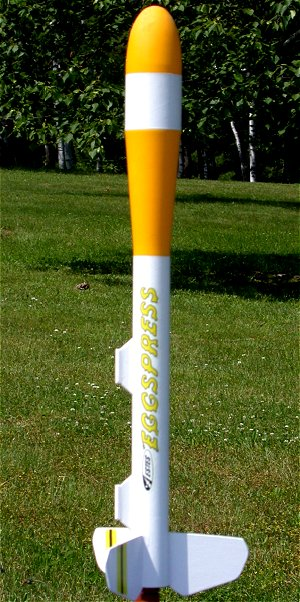
\includegraphics[width=0.2\textwidth]{1996_eggspress_zps43246419.jpg}
    \end{figure}

    \begin{figure}
      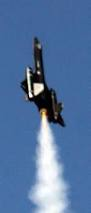
\includegraphics[width=0.2\textwidth]{SR71.jpeg}
    \end{figure}
    
    \column{0.45\textwidth}  
    \begin{itemize}
    \item Built model rockets as a kid and demoed them in school
    \end{itemize}
  \end{columns}
\end{frame}

\begin{frame}
  \frametitle{Electric Guitar Wiring}
  \begin{itemize}
  \item Dual coil humbucking pickups installed
  \item Installed combination potentiometer/DPDT switches for volume
    knobs
  \item Designed a circuit to allow phase switching and coil splitting
    via the switches
  \end{itemize}
  %% circuit diagram
  %% Network diagram  
\end{frame}

\begin{frame}
  \frametitle{Server Administration}
  \begin{itemize}
  \item Set up a low power headless Ubuntu server on Intel Celeron hardware
    \item Automated backup server
    \item Samba file server
    \item Plex media server
    \item Postfix mail server
    \item Home surveillance
  \end{itemize}
\end{frame}
\end{document}
